\documentclass[tcc]{subfiles}

\begin{document}

\chapter{Methods}
\label{sec:methods}
\epigraph{It's not denial. \\ I'm just very selective about the reality I accept.}{-Calvin}

This section deals with the models used for the engine compressor, turbine and nozzle, 
as well as the methods used for calculating the engine steady operation (engine matching), 
surge, dynamical behavior and performance parameters. 
Throughout this section, the ideal gas assumption is widely used, 
as is the assumption that the performance of a component can be separated in an ideal performance and a loss model. 
In the end, the engine from which the parameters for the model were extracted is described.

The component models are normally referred to as component maps or characteristic lines. 
A component map or characteristic is, in a general sense, the functional relationship between a component's
mass flow rate, rotation speed, pressure ratio and efficiency. 
These five unknowns are linked by two constraints, namely Euler's equation and a loss model. 
This leaves two free variables.
Usually compressor maps are plotted using the mass flow rate as the abscissa and  the pressure ratio as the ordinate, with contours for constant rotation speed and efficiency. 
For turbines, the rotational speed and efficiency is not uniquely defined for a combination of mass flow rate and pressure ratio. This led to the use of the artificial parameter of rotational speed times mass flow rate for the abscissa.

The name characteristic is most often used in reference to the iso-speed lines of a turbine or compressor when plotted in the plane of mass flow vs.\ pressure ratio.

Another way of plotting compressor maps is using the flow parameter as the abscissa and  the pressure rise or efficiency as ordinate. 
For incompressible flow this leads to the collapse of the constant rotational speed lines, thus being very convenient.


\section{Compressor model}

\subfile{text/body/compressor_map}


To write Euler's equation \cref{eqn:euler} in terms of the nondimensional parameters introduced in \cref{sec:nondimensional}, it suffices to rewrite $\phi_3$ and $\psi$ as a function of them. Thus
\begin{multline}
    \label{eqn:phi2_dimensionless}
    \phi_3 = \frac{W_{2r}}{U_3} 
           = \frac{\frac{\dot{m}}{\rho_3 A2}}{\acs{M0rotor} a_{02}}
           = \frac{\MFPalt{2}}{\acs{M0rotor}} \frac{a_{03}}{a_{02}} \stagdensratio{3} \\ 
           = \frac{\acs{MFP}_3}{\acs{M0rotor}} \sqrt{\frac{T_{03}}{T_{01}}} \stagdensratio{3}
\end{multline}
The value of $M_3$ can be obtained from $\acs{MFP}_3$ using \cref{eqn:mfp2mach}, while the latter is given by
\begin{equation}
    \label{eqn:mfp2mfp2}
    \acs{MFP}_3 \triangleq \MFP{2} = \acs{MFP} \frac{A_2}{A_3} \frac{P_{02}}{P_{03}} \sqrt{\frac{T_{03}}{T_{02}}}
\end{equation}
Notice that \cref{eqn:mfp2mfp2} makes no assumption of the process 1--2 being isentropic. $\acs{MFP}_3$ can be used along with \acs{MFP} to check for choking.

The load coefficient is given by
\begin{equation}
    \acs{load_coef}\triangleq \frac{\Delta h}{U_3^2}
                      = \frac{c_p(T_{02}-T_{02})}{U_3^2}
                      = \frac{\frac{c_p(T_{03}-T_{01})}{\gamma R T_{02}}}
                                    {\acs{M0rotor}^2}
                      = \frac{\frac{T_{03}}{T_{02}}-1}
                                  {\acs{M0rotor}^2}
                        \left(\frac{1}{\gamma-1}\right)
\end{equation}

At this point the loss models discussed in \cref{sec:compressor_losses} are introduced, 
and the values of $\acs{load_coef}_{\text{actual}}$ and $\acs{load_coef}_{\text{isen}}$ are obtained.
The temperature and pressure ratios can then be readily calculated from
\begin{align}
    \label{eqn:psi2Tratio}
    \frac{T_{03}}{T_{02}} &= (\gamma - 1)\psi_{\text{actual}} \acs{M0rotor}^2 + 1 \\
    \label{eqn:psi2Pratio}
    \frac{P_{03}}{P_{02}} &= \left[(\gamma - 1)\psi_{\text{isen}} \acs{M0rotor}^2 + 1\right]^\frac{\gamma}{\gamma-1}
\end{align}

In this work, only the losses due to incidence and skin friction were considered, because they are the ones most important for compressor stability (see \cref{sec:compressor_loss}). The model chosen for skin friction was suggest by \textcite{Oh1997} and the incidence losses where modeled as the complete conversion of all kinetic energy normal to be blade camber line to heat \cite{Galvas1973}. This is a more physical model than the one suggested by Oh et al., and captures better the loss variation with incidence, since Oh et al's model does not include flow angles. 


\section{Turbine model}
\subfile{text/body/turbine_map}

The turbine model is summarized in \cref{map:turbine}. 
Its development is mostly analogous to that of the compressor, with the exception of the loss and deviation models. 
Since the turbine does not exhibit flow instability phenomena such as compressor surge, 
which depends heavily on the incidence losses, 
and this work is focused on the dynamic modeling of the engine, 
the turbine was assumed isentropic. 
Nevertheless, a loss model based on pressure loss coefficients $Y_p$, $Y_s$, $Y_k$, etc.\ 
could easily be included in this model by modifying \cref{eqn:turb_res_pr} in the following way
\begin{equation}
    \frac{P_{05}}{P_{04}} -\frac{[1 + (\gamma-1)\psi_{\text{euler}} M_b^2]^{\frac{\gamma}{\gamma-1}}}{1+Y\left\{1-\left[1+\tfrac{\gamma-1}{2}M_5^2\right]^{-\frac{\gamma-1}{\gamma}}\right\}} = 0 
\end{equation}

where
\begin{equation}
    Y = Y_p + Y_s + Y_k
\end{equation}

This correction is derived as follows. The pressure loss coefficient is given by
\begin{equation}
    Y = \frac{P_{0i} - P_{0e}}{P_{0e} - P_e}
\end{equation}
Now we divide the numerator and the denominator by $P_{0e}$ and isolate the pressure ratio term 
\begin{equation}
    \frac{P_{0i}}{P_{0e}} = \frac{1}{1+Y\left\{1-\left[1+\tfrac{\gamma-1}{2}M_e^2\right]^{-\frac{\gamma-1}{\gamma}}\right\}}
\end{equation}
This pressure ratio loss term must be multiplied to the ideal (isentropic) pressure ratio given by the second term of \cref{eqn:turb_res_pr}. If more than one blade row is considered (e.g.\ one for the stator and another one for the rotor) the pressure ratio losses for each must be joined by multiplication.

\subfile{text/body/nozzle}


\section{Engine static model}

The engine static model, also known as steady state, 
describes the conditions in which the engine can operate indefinitely 
without changes in throttle input or outside conditions (pressure and temperature).

The engine model used is of the lumped volume type. This means that each component 
 (compressor, burner,turbine and nozzle)
 is modeled as a single point in space and conservation laws are applied to them.
 This type of model is also known as zero dimensional (0-D) or as parametric cycle analysis
 \index{parametric cycle analysis},
 and is widely used in both industry and academy as a tool for preliminary design and 
 performance analysis. 

A schematic of the engine components considered for the simulation of the present gas turbine engine is shown in \cref{fig:engine}.

\begin{figure}
    \caption{Schematic diagram of the modeled engine}
    \label{fig:engine}
    \includesvg{fig/engine_schematic}
    \source{\authorsfigure}
\end{figure}

Equations:
\begin{enumerate}
    \item Constant spool speed
    \item Conservation of energy transmitted through spool
    \item Conservation of mass in the burner
    \item Energy addition due to fuel
    \item nozzle
    \item turbine (x3)
    \item compressor (x3)
\end{enumerate}

\subfile{text/body/engine_map}

\subsection{Performance parameters}
\begin{itemize}
    \item thrust
    \item thermal efficiency
\end{itemize}

\section{Engine dynamical model}

\section{Surge model}

The model due to \textcite{Fink1988}, described in \cref{sec:review:surge} was adopted here. 
Since component matching is an important part of the surge mechanism, the engine matching model equations were mostly replicated here, with the exception of the nozzle equation since the exit pressure of the nozzle can be allowed to be arbitrary to consider all possible surge conditions. Surge will normally occur when the mass flow is severely reduced, which happens when the overall engine pressure ratio is big. This equation was replaced by Fink's stability criterion \cref{eqn:surge}. The resulting model is in \cref{model:surge} \todo{add table with model formulation}.

\section{Numerical aspects}

As was shown in this section, the models for a gas turbine engine and its components are expressed naturally in the form of coupled (sometimes differential) non-linear systems of equations. 
These systems are inherently coupled because their behavior depends on the flow angles on both the inlet and exit, and these can not be calculated independently of one another.
As discussed in \cref{sec:review:numeric}, these problems are examples of \ac{DAE} systems, and many of them do not have explicit derivatives in their formulation.

In this section, the numerical approach used to calculate each of the models described in this chapter will be exposed. They consist of a mix of nonlinear solvers, namely Powell's hybrid method and Levenberg-Marquardt, as implemented by \textsc{minpack} and available in the Python package scipy, and of the newer \ac{DAE} solver \textsc{IDA}, available as part of \textsc{sundials} \cite{sundials} with a Python interface by Assimulo \cite{assimulo}.

\subsection{Generation of component maps}
Nonlinear solver (hybr or lm) coupled with a breadth-first search. Initial point in the $x$ and $y$-axis is chosen randomly within the choke boundaries, pressure and temperature ratios are unit, mach numbers are between 0 an 1. If convergence is achieved a breadth-first search considering that each point in the grid is a graph node connected to the points up, down, left, right and in the diagonals. The converged result for each point is used as an initial guess for neighboring points. This allows each point in the grid up to 8 different initial guesses quite close to the actual solution (if the grid is fine enough), and has proven very robust. 

\subsubsection*{Choke line}
Compressor: find point where inlet and exit are simultaneously choked. For pressure ratios above this critical value, only the inlet is choked and the choke line is vertical. For pressure ratios bellow this value the exit is choked. The choke line was verified to be a straight line, so that just the point at another pressure ratio, e.g.\ the minimum pressure ratio of interest (normally unit) is needed to fully define it.

Turbine: it is linear in a plot of \acs{MFP} vs.\ pressure ratio, but in this case the blade mach number is not uniquely defined. In a plot of $\acs{MFP}M_b$ vs.\ expansion ratio, the choke line is nonlinear and a KS aggregation function with variable $rho$ was added to the turbine model to model the choke.

\subsection{Generation of the working line}
Optimize the engine model for maximum efficiency.
Then use a \ac{DAE} solver to continue the line forwards and backwards.

\subsection{Dynamical simulation}
Use a \ac{DAE} starting from an equilibrium (static) point.
Inputs: step in T04 up and down; senoids?

\section{The VT-80 engine}
The engine chosen to which apply these models was Jet-Munts VT-80.
This engine was developed for hobby use in airplane models and comes with an \gls{ECU} installed from factory, which will not be used for this work.
It is a single spool jet engine, with a single stage centrifugal compressor 
 and also single stage axial turbine, as seen in \cref{fig:engine}. 
It runs on aviation kerosene premixed with oil.%
The specifications provided by the manufacturer are in \cref{tbl:engine_specs}.
\textcite{bolsoni} estimates the compressor pressure ratio 
to be around 2.2 based on similar engines.

\begin{figure}[p]
    \centering
    \caption{JetsMunt VT-80 jet engine}
    \label{fig:engine}
    \begin{subfigure}{\textwidth}
        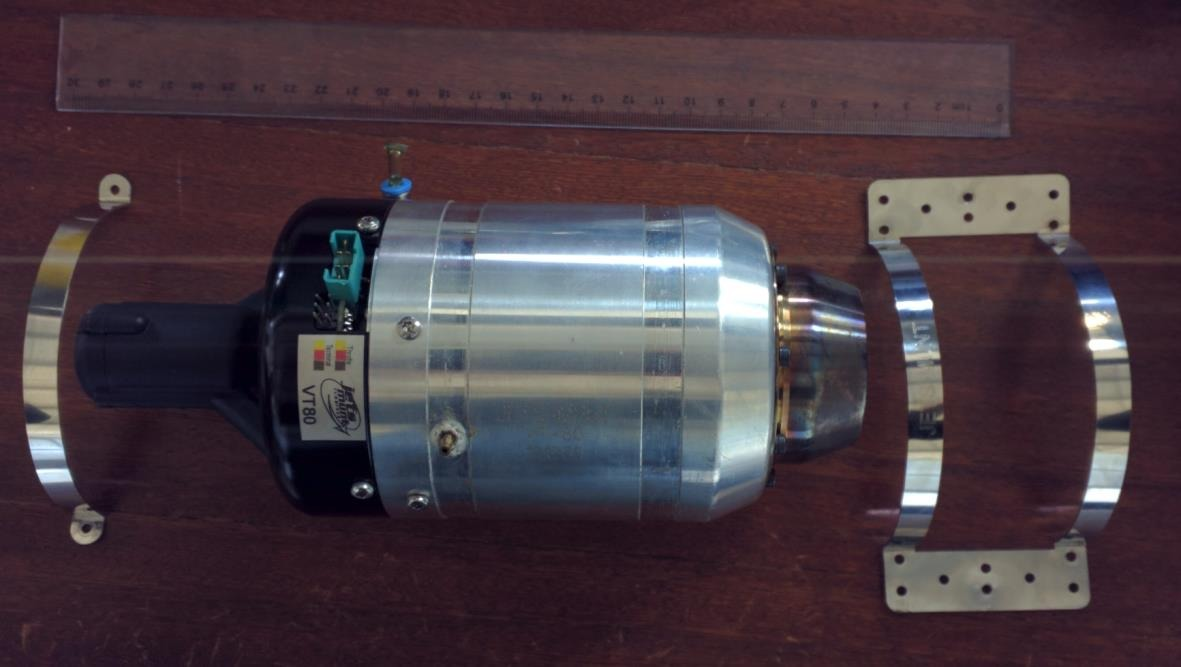
\includegraphics[width=\textwidth]{fig/JetsMuntVT-80.jpg}
        \caption{Picture with a 30cm ruler for scale}
        \label{fig:engine!visible}
    \end{subfigure}
    \begin{subfigure}{\textwidth}
        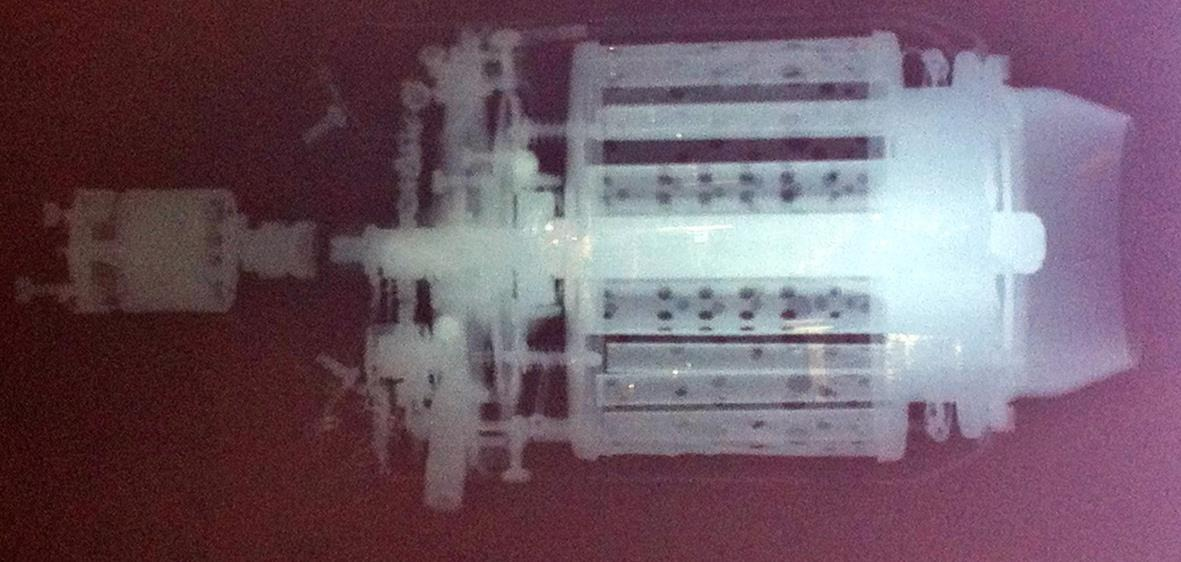
\includegraphics[width=\textwidth]{fig/JetsMuntVT-80X-ray.jpg}
        \caption{X-ray picture}
        \label{fig:engine!x-ray}
    \end{subfigure}
    \source{\cite{bolsoni}}
\end{figure}

\begin{table}
    \centering
    \caption{VT80 Specifications}
    \label{tbl:engine_specs}
    \begin{tabular}{lr@{$\,$}l}
        \toprule
        Diameter (external)                & 90 & mm \\
        Length                             & 240 & mm \\
        Weight (bare)                      & 950 & g \\
        Weight (with accessories)          & 1075 & g \\
        Nominal thrust @ 15C and sea level & 80 & N \\
        Idle thrust                        & 4 & N \\
        Max rpm                            & 150 000 & rpm \\
        Idle rpm                           & 45 000  & rpm \\
        Heat soak rpm                      & 12 000  & rpm \\
        \acs{EGT} @ max rpm                & 600$\pm$50 & \si{\celsius} \\
        Fuel consumption @ max rpm         & 0.29 & L/min \\
        Fuel/oil                   &\multicolumn{2}{l}{Kerosene + 4\% oil} \\
        \bottomrule
    \end{tabular}
    \source{\cite{engine-manual}}
\end{table}

\todo{geometrical engine parameters used in simulation}

\end{document}
